
\chapter{System design}
\section{System overview} \label{sec:system}

\begin{figure}[h]
    \centering
    \vspace{-0.7cm}
    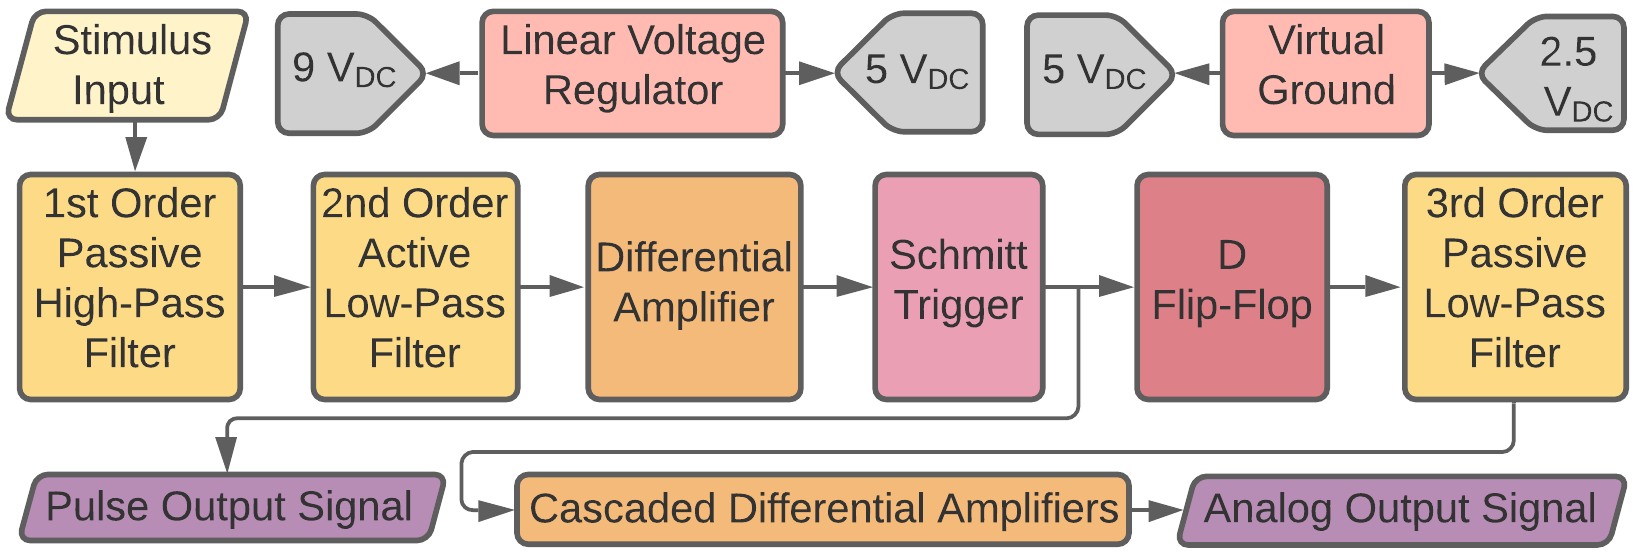
\includegraphics[width = 1\textwidth]{Figures/overview}
    \caption{System Diagram}
    \label{fig:overview}
\end{figure}

Creating a health monitoring system requires the design and implementation of a heart-rate sensor. This sensor obtains an input signal, from which pulses, corresponding to heart-beats are generated, as well as analogue values which represent the heart-rate. The aforementioned is achieved by means of various subcircuits, respectively responsible for voltage regulation, signal conditioning, pulse generation and conversion to analogue, which proceeds as can be seen in figure \ref{fig:overview} - explanation follows hereafter.
A voltage regulator generates 5 V which powers the circuit. See \ref{ } old report for the design. The stimulus input signal, obtained from the heart-rate sensor, is to be converted to a pulse output signal, but has an amplitude of insufficient magnitude, and is subject to high levels of noise. This necessitates signal conditioning: the input signal is fed into a first order passive high-pass filter and a second-order active low-pass filter consecutively, thereby attenuating both high- and low-frequency noise. The filters were chosen with maximal simplicity in mind, as to reduce cost and complexity, while still performing adequately. After filtering, the signal is amplified by means of a differential amplifier, resulting in a signal with a large amplitude and little noise. This allows for pulse generation by means of a Schmitt Trigger comparator, which produces an output pulse signal, where the frequency corresponds to the heart-rate. The Schmitt Trigger was preferred above alternatives as it provides a a noise margin by means of hysteresis, thereby eliminating heart-beat misdetections that otherwise arise. Further, an analogue voltage is required, where the voltage level represents the heart-rate. Filtering and peak detection using diodes was considered, but ultimately discarded, as diodes are non-linear, resulting in extremely slow simulation. Rather, the pulse output signal was converted to a pulse-width modulated signal, where the frequency of the former determined the duty cycle of the latter. This was done as PWM signals lend themselves to conversion-to-analogue by simple filtering. The PWM signal was obtained by using a D Flip-Flop in conjunction with a RC-circuit (see section \ref{•} for more detail), and was then filtered by a fourth-order passive RC filter. Passive components were selected as to reduce current usage and simulation time. The filter is of high order as to greatly minimize noise, as the settling time requirement for the analog signal was easily met.

\pagebreak


Also point the reader to your first report for more information on the temperature sensing and voltage regulation, and use a citation to it (add it to your \texttt{References.bib} file and cite it here). Remember to state what your remaining power budget is, based on Assignment 1's results. 








